\section{Entraînement et évaluation des modèles pour les données network}
 
Pour cette partie nous avons décider de présenter le modèle KNN sur le dataset numéro 1 et les autres méthode sur le dataset numéro 4. Nous avons fait ce choix car ce sont les résultats les plus intéressant que nous avons obtenu. 

\subsection{KNN (K-Nearest Neighbors)}

Ici nous avons aussi conclu avec la même méthode du meilleurs \(k\) pour le modèle KNN. Nous avons trouvé que le meilleur \(k\) est 5. Nous avons donc entraîné le modèle KNN avec \(k = 5\).

Le modèle KNN atteint une précision globale de 0.89, indiquant des performances globalement satisfaisantes. Cependant, une analyse détaillée des métriques par classe révèle des disparités notables. La classe majoritaire "normal" est parfaitement prédite avec une précision, un rappel et un F1-score de 1.00, ce qui reflète la capacité du modèle à gérer efficacement les données dominantes. En revanche, les classes minoritaires, notamment "physical fault", présentent des performances significativement inférieures, avec un F1-score de seulement 0.39 dû à une faible précision (0.52) et un rappel (0.32). Cela suggère que le modèle a des difficultés à identifier correctement cette classe, probablement en raison d'un déséquilibre dans les données ou d'une proximité élevée entre les instances de différentes classes dans l'espace des caractéristiques.

La classe "MITM" affiche des performances intermédiaires, avec un F1-score de 0.77, soutenu par un rappel de 0.84, ce qui indique que le modèle détecte correctement la plupart des cas, bien que des erreurs subsistent.

\begin{figure}[H]
    \centering
    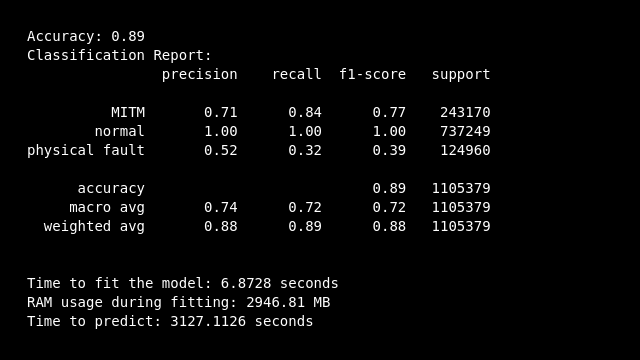
\includegraphics[width=0.8\textwidth]{figures/training/res_KNN.png}
    \caption{Résultats du modèle KNN avec \(k = 5\) pour le dataFrame 1}
    \label{fig:knn}
\end{figure}

\subsection{CART (Classification And Regression Tree)}

Le modèle CART (\textit{Classification and Regression Tree}) atteint une précision globale de 0.96, témoignant d'excellentes performances générales. Les métriques par classe montrent une capacité robuste à prédire les étiquettes majoritaires. La classe "normal", qui constitue la majorité des données, est parfaitement prédite avec un F1-score de 1.00, de même que la classe "scan", bien que cette dernière ait un faible support de seulement 6 instances.

Les performances sur les classes minoritaires, comme "physical fault", sont légèrement inférieures avec un F1-score de 0.70, une précision de 0.75, et un rappel de 0.66, ce qui indique que le modèle confond parfois cette classe avec d'autres. La classe "MITM" est mieux prédite, avec un F1-score de 0.82 et un rappel de 0.84, démontrant une bonne capacité à détecter les anomalies de ce type. La classe "DoS" affiche d'excellents résultats, avec un F1-score de 0.99 et un rappel parfait de 1.00.

La matrice de confusion révèle que le modèle a tendance à confondre les classes "physical fault", "MITM" et "DoS", ce qui explique les performances relativement faibles sur ces classes. Cela suggère que ces classes sont difficiles à distinguer dans l'espace des caractéristiques.


\begin{figure}[H]
    \centering
    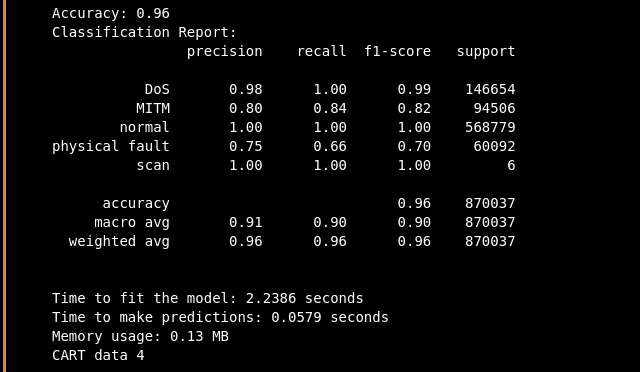
\includegraphics[width=0.8\textwidth]{figures/training/res_cart.png}
    \caption{Résultats du modèle CART pour le dataFrame 4}
    \label{fig:cart_res}
\end{figure}

\begin{figure}[H]
    \centering
    \includegraphics[width=0.8\textwidth]{figures/training/confusion_CART.png}
    \caption{Matrice de confusion du modèle CART pour le dataFrame 4}
    \label{fig:cart_matrix}
\end{figure}

\subsection{Random Forest}

Le modèle Random Forest atteint une précision globale de 0.96, identique à celle obtenue avec le modèle CART, et montre des performances similaires sur les classes majoritaires et minoritaires. Comme pour CART, la classe "normal" est parfaitement prédite avec un F1-score de 1.00, et la classe "scan", malgré son faible support (6 instances), est également prédite avec une précision et un rappel parfaits.

Pour les classes minoritaires, les résultats de Random Forest sont presque identiques à ceux de CART. La classe "physical fault" obtient un F1-score de 0.70, avec une précision de 0.74 et un rappel de 0.66, ce qui reflète des performances équivalentes à celles du modèle CART. De même, la classe "MITM" affiche un F1-score de 0.82 et un rappel de 0.84, soulignant une capacité comparable des deux modèles à détecter cette classe.

\begin{figure}[H]
    \centering
    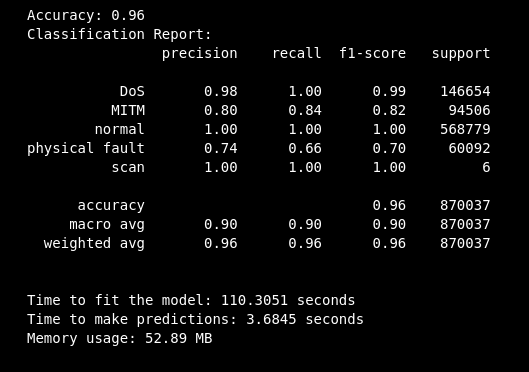
\includegraphics[width=0.8\textwidth]{figures/training/res_random_forest.png}
    \caption{Résultats du modèle Random Forest pour le dataFrame 4}
    \label{fig:rdf_res}
\end{figure}

\begin{figure}[H]
    \centering
    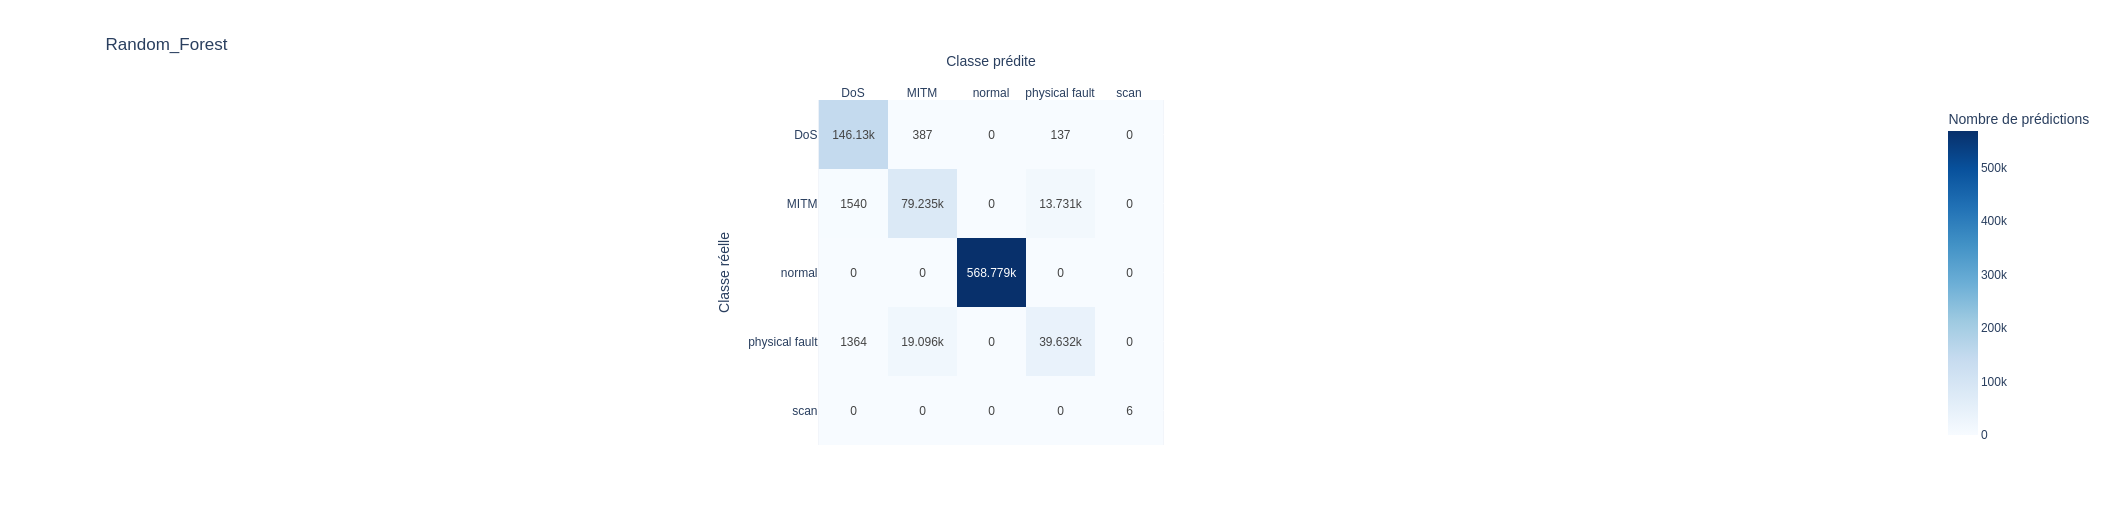
\includegraphics[width=0.8\textwidth]{figures/training/Confusion_random_forest.png}
    \caption{Matrice de confusion du modèle Random Forest pour le dataFrame 4}
    \label{fig:rdf_matrix}
\end{figure}


\subsection{XGBoost (Extreme Gradient Boosting)}

Le modèle XGBoost atteint une précision globale de 0.95, légèrement inférieure à celle des modèles CART et Random Forest, qui atteignent tous deux une précision de 0.96. Pour les classes majoritaires comme "normal", XGBoost conserve un F1-score parfait de 1.00, comparable aux deux autres modèles, montrant une excellente capacité à traiter les classes dominantes. De même, la classe "scan", bien que peu représentée (6 instances), obtient un F1-score de 0.80, une performance inférieure à CART et random forest.

Les performances sur les classes minoritaires révèlent des différences significatives. Pour la classe "physical fault", XGBoost obtient un F1-score de 0.60, inférieur à celui de Random Forest et de CART (0.70), avec un rappel particulièrement faible de 0.53. La classe "MITM" montre des résultats intermédiaires avec un F1-score de 0.77, inférieur à celui de Random Forest (0.82) et de CART (0.82). Ces résultats indiquent que XGBoost a davantage de difficultés à prédire correctement ces classes par rapport aux deux autres modèles.

\begin{figure}[H]
    \centering
    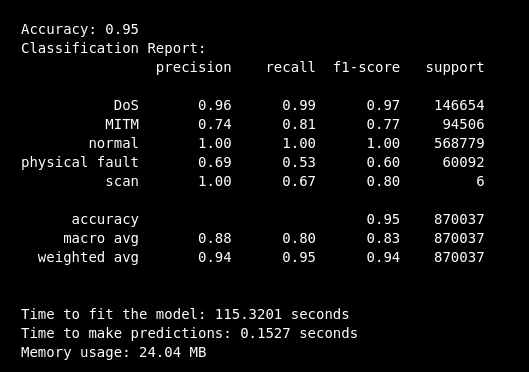
\includegraphics[width=0.8\textwidth]{figures/training/res_XGBOOST.png}
    \caption{Résultats du modèle XGBoost pour le dataFrame 4}
    \label{fig:rdf_res}
\end{figure}

\begin{figure}[H]
    \centering
    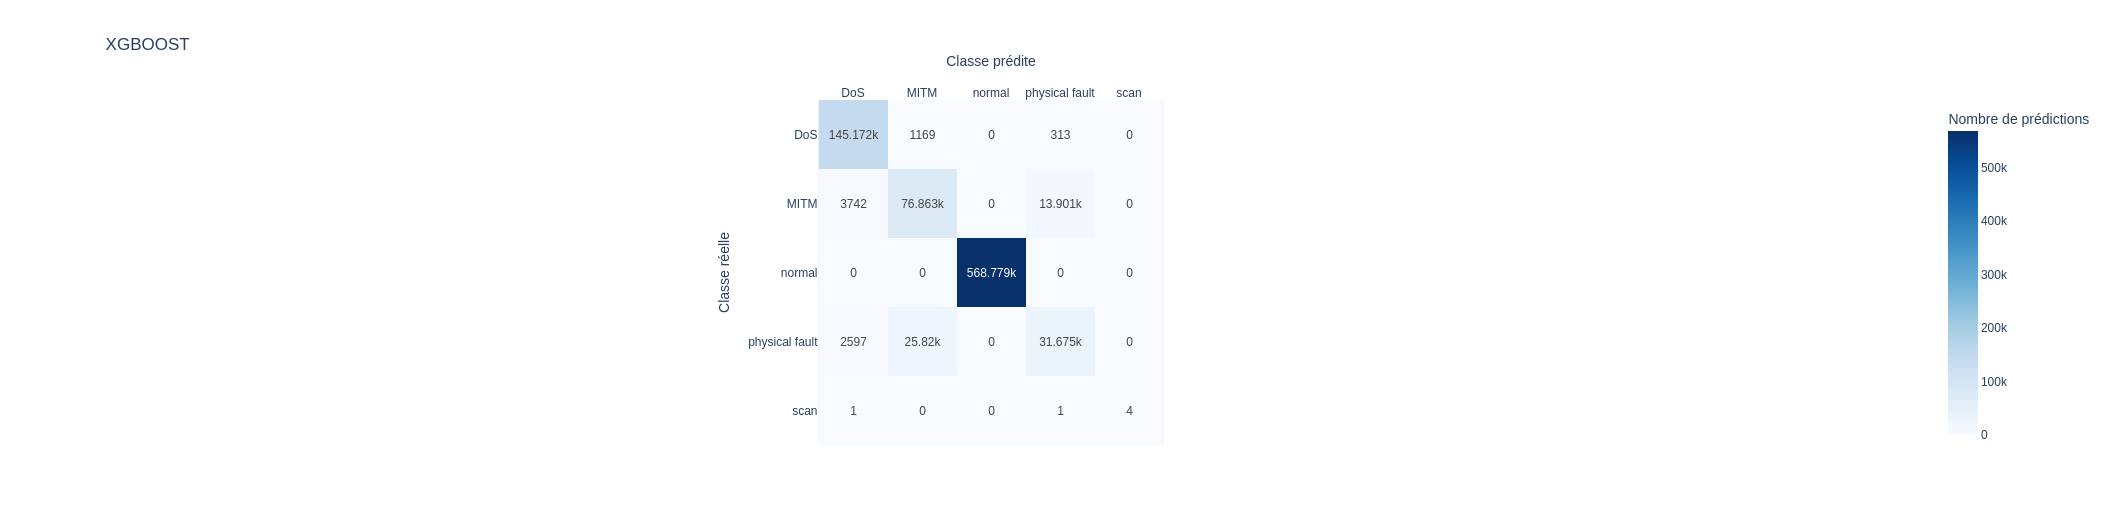
\includegraphics[width=0.8\textwidth]{figures/training/Confusion_XGBOOST.png}
    \caption{Matrice de confusion du modèle XGBoost pour le dataFrame 4}
    \label{fig:rdf_matrix}
\end{figure}